\documentclass[12pt,a4paper,oneside,english]{book}

\usepackage{cite}


%\usepackage[latin1]{inputenc}

%\usepackage[T1]{fontenc}
\usepackage[english]{babel}
\usepackage{amsmath}
\usepackage{amsfonts}
\usepackage{amssymb}
\usepackage{graphicx}
\usepackage{subfig}
\usepackage{fancyhdr}
\usepackage{appendix}
\usepackage{hyphenat}
\usepackage{pdfpages}
\usepackage{svg}

%\usepackage{tocloft} % For TOC customization ( table of contents )
\usepackage{array,multirow,makecell}
\newcolumntype{C}[1]{>{\arraybackslash}p{#1}}

\usepackage{enumitem}
\setlist{leftmargin=*,itemsep=0pt}

\usepackage{centernot}
\usepackage[linesnumbered,ruled,vlined,english,onelanguage]{algorithm2e}

\usepackage{quotchap}
\makeatletter
\renewcommand{\@makechapterhead}[1]{
 \chapterheadstartvskip
 {\size@chapter{\sectfont\raggedright
 {\chapnumfont
 \ifnum \c@secnumdepth >\m@ne
 \if@mainmatter\thechapter %frontmatter for roman numerals
 \fi\fi
 \par\nobreak}
 {\raggedright\advance\leftmargin10em\interlinepenalty\@M #1\par}}
 \nobreak\chapterheadendvskip}}
\makeatother
\renewcommand*{\chapterheadendvskip}{\vspace{2cm}}
%\renewcommand{\thechapter}{\Roman{chapter}} % Set chapter numbering to Roman numerals


\usepackage{geometry}
\geometry{hmargin=2cm,vmargin=2cm}

\pagestyle{fancyplain}
\lhead{\fancyplain{}{\nouppercase{\textit{\leftmark}}}}
\chead{\fancyplain{}{}}
\rhead{\fancyplain{}{}}
\lfoot{\fancyplain{}{}}
\cfoot{\fancyplain{}{}}
\rfoot{\fancyplain{\thepage}{\thepage}}
\renewcommand{\headrulewidth}{1pt}
\renewcommand{\footrulewidth}{1pt}

\renewcommand{\thesection}{\Roman{section}} % Set section numbering to Roman numerals % previously \arabic{section}

\usepackage{titlesec}
\titleformat{\paragraph}{\fontsize{11}{10}\bfseries}{\theparagraph}{1em}{}
\titlespacing*{\paragraph}{0pt}{10pt plus 2pt minus 0pt}{0pt plus 2pt minus 0pt}

\setcounter{secnumdepth}{4}
\setcounter{tocdepth}{4}

%%%%%
\usepackage{listings}
\usepackage{xcolor} % Required for colors

% Define a custom style for JSON
\lstdefinestyle{jsonstyle-compact}{
    language=Java, % listings doesn't have a JSON language, but Java is close enough
    basicstyle=\footnotesize\ttfamily, % Use a smaller font
    keywordstyle=\color{blue},
    stringstyle=\color{black},
    commentstyle=\color{green},
    morestring=[b]",
    showstringspaces=false,
    breaklines=true,
    frame=none, % Remove the frame/rectangle
    backgroundcolor= \color{gray!5} %{gray!10}
}
%%%


\usepackage{array}
\usepackage{multirow}
%\addto\captionsfrench{\def\tablename{\textsc{Tableau}}}

%\DefineBibliographyStrings{french}{urlseen = {},}

\setlength{\parskip}{0pt}%was 8 : space between paragraphs
\setlength{\parindent}{1.5em}%was 1.5 : indentation of paragraphs

\usepackage{setspace}

\usepackage{url}

\usepackage{hyperref}
% Comment before printing to remove links' colors
\definecolor{darkblue}{rgb}{0.0, 0.0, 0.5}
\hypersetup{
 colorlinks,
 linktocpage=true,
 linkcolor={darkblue},
 citecolor={darkblue},
 urlcolor={blue}}

\sloppy

\author{You}
\title{Internship Report}

\begin{document}
\pagenumbering{gobble}
\includepdf[pages=-]{FrontPage.pdf}
\chapter*{Acknowledgments}

\frontmatter %here yothhrou les num des pages en bas 
\chapter*{Abstract}
\normalsize{Write your abstract here.

\medskip
{\noindent \textbf{Keywords: ..., ... .} }

\spacing{1}
\tableofcontents{}
\newpage 
\listoffigures
\newpage 
\listoftables
\newpage
\spacing{1.4}
\chapter*{List of acronyms}
%\addcontentsline{toc}{chapter}{Liste des acronymes}
\markboth{List of acronyms}{}%abbrev
\begin{itemize}
\item \textbf{AI} Artificial Intelligence
\item \textbf{ML} Machine Learning
\item \textbf{API} Application Programming Interface
\item \textbf{ASR} Automatic Speech Recognition
\item \textbf{SER} Speech Emotion Recognition
\item  \textbf{NLP} Natural Language Processing
\item \textbf{DBSCAN} Density-Based Spatial Clustering of Applications with Noise
\item \textbf{GIS} Geographical Information System
\item \textbf{GPS} Global Positioning System
\item \textbf{BERT} Bidirectional Encoder Representations from Transformers
\end{itemize}

\frontmatter %here yothhrou les num des pages fl contnent
%\frontmatter  %to have roman page numbering in the beginning
%\mtcaddchapter[Introduction g�n�rale]

\chapter*{Introduction}
\addcontentsline{toc}{chapter}{Introduction}
\markboth{Introduction}{}

\chapter{Company Presentation} % we should metion that there are a lot of spacing between title of chapter and sctions

\label{ch:1er}
\section{Overview}
Founded in 2020, and located in both Meudon la forêt , Meudonn France and tunis, Tunisia, 
Hydatis is dedicated to helping early-stage companies leverage the latest data intelligence and digital technologies to solve real-world challenges, becoming, since then, a leading technology startup studio with a proven track record.
\begin{figure}[h!] % placement options: h=here, t=top, b=bottom, p=page
    \centering
    
\includegraphics[width=0.2\textwidth]{images/hydatiss.png}
    \caption{Logo of Hydatis}
    \label{fig:hydatis}
\end{figure}

Hydatis specializes in AI, machine learning, blockchain, big data Analysis and more. Hydatis's team of technology experts is dedicated to building scalable and sustainable businesses, with a focus on creativity, strategy, and technology alongside with a vast network of partners and investors and a strong reputation in the technology industry.
\begin{figure}[h!] % placement options: h=here, t=top, b=bottom, p=page
    \centering
    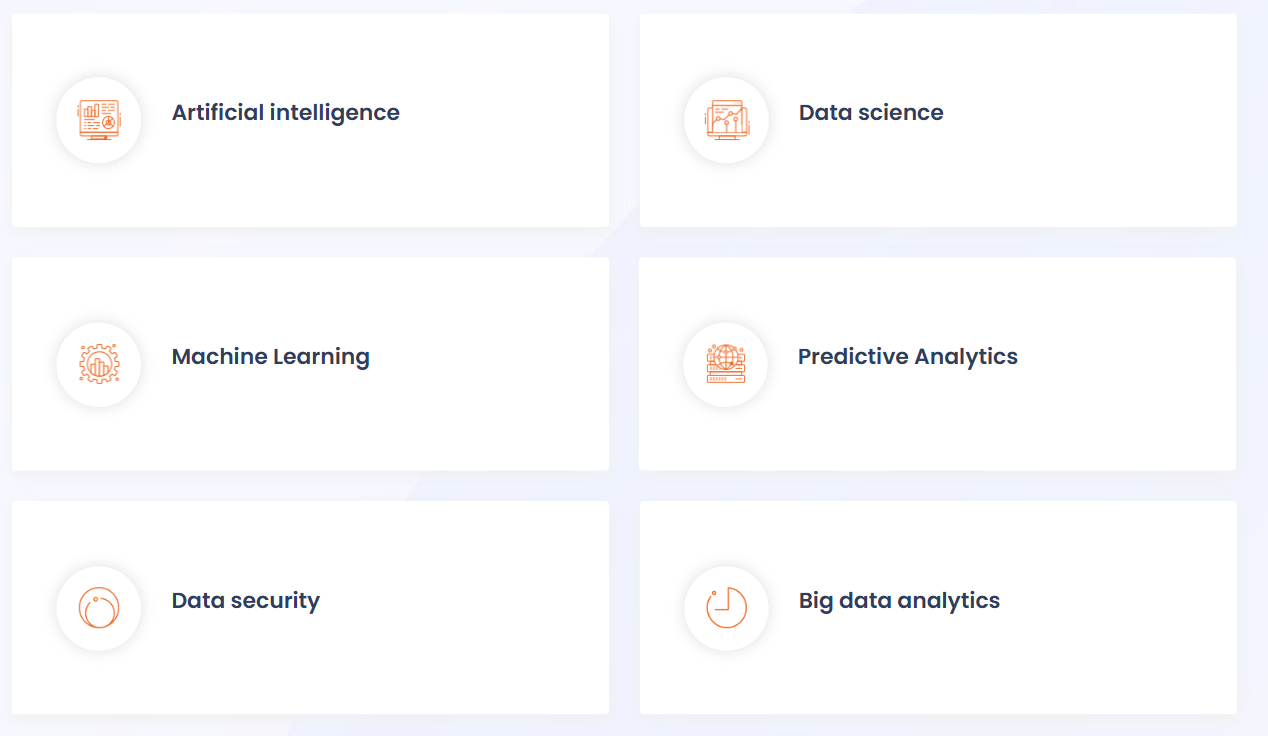
\includegraphics[width=0.699\textwidth]{images/Expertise_hydatis.png}
    \caption{Hydatis' Areas of Expertise}
    \label{fig:Expertise_hydatis}
\end{figure}

\section{Sectors of Activities}%and services offered
Hydatis is a product-focused Tech venture studio offering a range of services tailored to the unique needs of each startup, including:
 business planning, product development, marketing, and fundraising. 
%With their expertise in data analytics, machine learning, and other advanced technologies, 
Leveraging technology and entrepreneurship, they help clients turn data into actionable insights that drive business success.
%help businesses make big decisions about their future by making tangible versions of tomorrow.
\subsection{Services offered}
\begin{itemize}
    \item \textbf {Software development Services}
    \item \textbf{CTO as a service}
    \item \textbf{IT Consulting}
    \item \textbf{Devops Consulting}
    \item \textbf{and a lot more...}
\end{itemize}
\begin{figure}[h!]
    \centering
    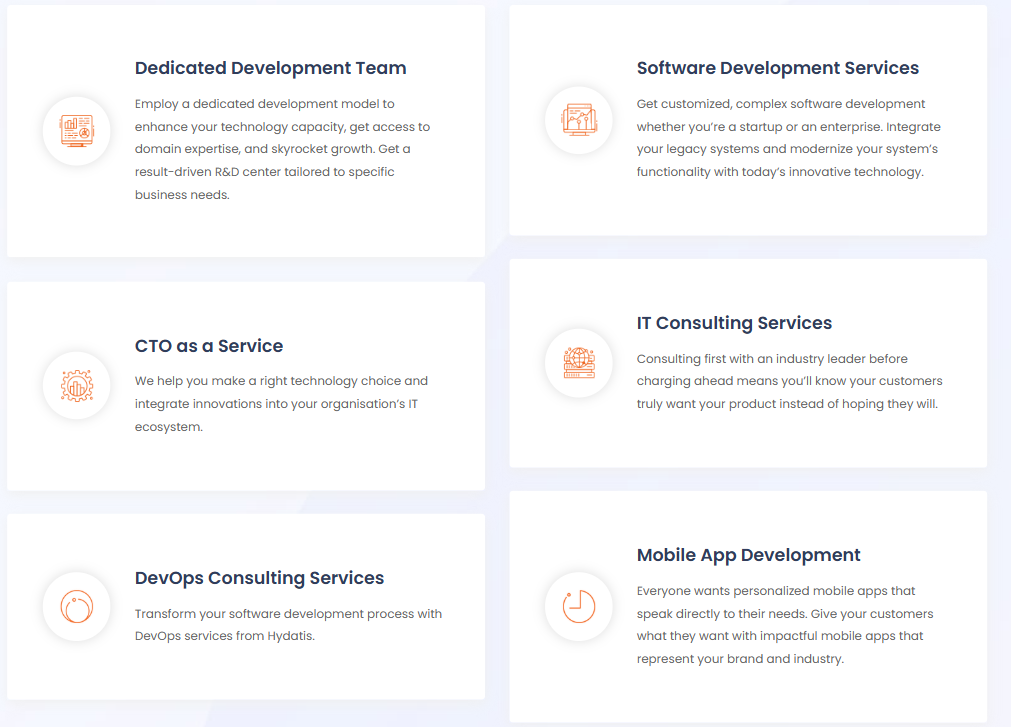
\includegraphics[width=0.9\textwidth]{images/services_hydatis.png}
    \caption{Hydatis' Services}
    \label{fig:Services_hydatis}
\end{figure}

\section{Organizational structure and Human Capital} % eithr this part will be deleted or the susection in the activities section will be modified and either discard items or having an individual subsection
Hydatis with a flat organizational structure that reflects its startup studio roots, led by  expertised directors who drive strategy and innovation alongside a talented crew of entrepreneurs and technologists, business strategists and network coordinators.

From AI specialists shaping cutting-edge products to strategists securing partnerships, and sicne its launch in 2020, these folks, with their varied backgrounds, suceeded to make Hydatis a powerhouse in the startup ecosystem.


\chapter{Internship Context and Objectives}
\label{ch:2eme}
\section{Problem Statement and Motivation} %Why
Crime is a major social problem in Tunisia, threatening public safety and disrupting the economy,ranging from theft to harassment, often leaving individuals vulnerable, especially at night or in isolated spots.
 
Traditional safety solutions such as manual reporting or basic wearable alarms have served as a foundational step in personal security. However they %struggle
suffer from critical limitations: 
The binary nature of a simple button press is usually unsufficient to distinguish between 
a genuine, life-threatening emergency,a false alarm, or a low-priority situation.
Additionally, the lack of contextual awarness results in inaccurate alerts and overwhelming emergency services with false positives. %Inaccuracy and Context Deficiency:
Giving the limited resources of emergency services (police, paramedics), false alarms divert critical attention away from genuine crises, incurring unnecessary costs and potentially delaying responses to real incidents. %Resource Depletion:


%The binary nature of a simple button press: unsufficient to distinguish between 
%a genuine, life-threatening emergency,a false alarm, or a low-priority situation. This leads to an unacceptably 
%high rate of false positives.

%  This gap hits home for Hydatis, the motivation behind this work is clear: we need to move beyond simple, reactive triggers
% and build smarter, faster ways to protect people by qualifying alerts with precision.
\subsection{Market Context and Existing Solutions}

Several commercial solutions exist in the personal safety market, including panic button apps like 
bSafe, location-sharing platforms like Life360, and wearable devices such as personal alarms. However,
 these solutions typically operate independently and lack the intelligent analysis needed to 
 differentiate between genuine emergencies and false alarms and ensure fast response to threats. 
 %, leading to the limitations described above.
Therefore, there is a clear need for an intelligent safety system that can analyze multiple data 
streams—location, audio, and behavioral patterns—to provide accurate, context-aware emergency 
detection while minimizing false positives.

%In State of the Art, you can include:
%Existing products (apps, devices, services → e.g., SOS apps, smartwatches with panic buttons, crime reporting platforms).
%Research/technical approaches (papers on anomaly detection, crime prediction models, wearable safety devices).
%Limitations of these (false positives, lack of contextual awareness, poor adoption, battery issues, limited reach, etc.).

%Detailed technical comparisons
%Algorithm discussions
%Academic literature reviews
%In-depth analysis of existing methods

%todo: reduce space in the footer ( especially see this page!)
%todo: and fama paget fihom khatt fl footer o whayed lee

\section{Description}% or scope : the "What." and "how" A high-level overview of the solution.

This project involves designing an AI-powered module for a Smart wearable Solution, aimed at enhancing personal safety through automated incident detection during my Summer internship at Hydatis.
The module integrates four key data streams: 
\begin{itemize}
    \item \textbf{Geospatial Analysis:} geospatial data derived from Tunisian crime datasets to identify high-risk areas.
    \item \textbf{Vocal Signal Processing:}  real-time vocal analysis to detect distress signals or key words such as calls for help.
    \item \textbf{Behavioral Profiling:} behavioral patterns to flag anomalies in user activitythat may indicate danger.
    \item \textbf{Decision Engine:} later, these components are fused into a cohesive system that processes and combines 
insights from each stream, offering a foundation for reliable alert qualification.
\end{itemize}
Though, detailed implementation will be explored in later sections.


\section{Core Mission, Objectives and Expected Results}

\subsection{Core Mission}
My core mission in this project is to develop an intelligent, multi-modal safety system that integrates  geospatial analysis, vocal processing, and behavioral profiling to transform personal security and  provide accurate , context-aware emergency detection that minimizes false alarms while ensuring genuine immediate attention to genuine threats  .

\subsection{Main Objectives}

\textbf{Technical Objectives:}
\begin{itemize}
    \item Achieve a minimum of 80\% accuracy in alert qualification.
    \item Minimize false positive rates. 
    \item Enable real-time processing  with response times under 5 seconds.
    \item Design a robust system capable of handling diverse scenarios and user behaviors.
\end{itemize}

\textbf{Implementation Objectives:}
\begin{itemize}

\item Process a Tunisian crime dataset for geospatial risk assessment.
\item Train a vocal ASR model adapted to Tunisian dialects for distress-related risk detection.
\item Prepare a vocal pipeline to analyse vocal patterns including: tone, rythm, and pitch.
\item Design a comprehensive database of processed behavioral patterns for every user.
   \item Integrate three distinct AI modules (geospatial, vocal, behavioral) into a cohesive system.
    \item Develop a proof-of-concept API for periodic risk assessment and scoring alerts.
    \item Ensure system scalability for potential deployment beyond Tunisia.
\end{itemize}

\subsection{Expected Results}
\begin{itemize}
\item A cleaned and structured Tunisian crime dataset inferred to geospatial risk analysis.
\item An ASR model integrated for vocal analysis in tunisian Arabic. %supporting real-time distress detection.
\item A vocal pipeline capable of analysing vocal patterns of stress and/or fear.
\item ML models designed for inferring  users behaviors.
\item A proof-of-concept multi-modal scoring system with sub-5-second responses.
\item APIs developed for periodic risk assessment and potential integration into a mobile or web interface.
\end{itemize}


\section{Internship timeline }% or planning %professionalism and project management skills.%%%%%often a Gantt chart)
%Timeline = just dates and deadlines
%Planning = timeline + methodology + resources + milestones

This project is structured over my two-month internship period at Hydatis, devided into:
\begin{itemize}
    \item \textbf{Weeks 1-2:} Initial research, dataset acquisition, and preprocessing.
    \item \textbf{Weeks 3-4:} Development of the geospatial analysis module and initial vocal processing pipeline.
    \item \textbf{Weeks 5-6:} Behavioral profiling model development and integration of the three AI modules.
    \item \textbf{Weeks 7-8:} Final system integration, testing, optimization, and documentation.
\end{itemize}

%todo: label the sections and subsections
%todo: diagramme de gantt!!!!

\chapter{Theoritical Foundations and State of the Art}
\label{ch:3eme}

% normalement we should put here:  State of the Art and Market Solutions section
% or subsection in the motivation and problem statement section: Existing Solutions and Limitations”
\section*{Introdunction}
This chapter presents the theoretical foundations underlying the proposed multi-modal safety system, which integrates three distinct yet complementary technologies:

First, the principles of geospatial analysis for risk prediction will be examined. 
Second, the field of vocal signal processing for distress detection will be explored, detailing the methods used to identify audible signs of an emergency from a user's speech. 
Finally, the concepts of machine learning applied on behavioral anomaly detection will be discussed, explaining the detection of anomalies based on personal routines.
\\This review justifies the technical choices made in the subsequent implementation chapter.
%establishes the scientific basis for
\section{Geospatical Analysis for Risk Prediction}
\label{sec:geospatial_theory}

Geospatial analysis integrates Geographical Information Systems (GIS) with advanced analytical techniques to identify crime hotspots, cluster incidents, and enable real-time risk assessment. This section explores hotspot forecasting, density-based clustering, and the evolution toward real-time systems, aligning with the need for intelligent personal safety solutions.

%This section establishes the theoretical foundations for location-based risk assessment module, which forms a core component 
%of the proposed multi-modal safety system.
%The analysis begins with crime hotspot theory and spatial clustering principles. Subsequently, density-based clustering algorithms, 
%particularly DBSCAN, are examined. Finally, the transition from static crime mapping to real-time risk assessment systems is explored.


\subsection{Crime Hotspot Forecasting and Spatial Analysis}


%Geospatial anomaly detection leverages Geographical Information Systems (GIS) to identify unusual patterns in spatial data, 
%a critical step in predicting crime hotspots. GIS integrates spatial datasets—such as crime locations, demographic details, 
%and environmental factors—into a unified framework for analysis [El-Fishawy et al., 2024]. 
%W ANTED TO PUT IT HERE

The foundational principle of crime hotspot analysis is that criminal activity is not randomly 
distributed, but rather concentrated in specific areas known as 'hotspots'
This involves analyzing geographic patterns where crime incidents cluster,
often influenced by factors like urban density or offender homogeneity \cite{chen2019exploring}. 
Hotspot theory posits that such clusters represent areas of elevated risk, necessitating targeted interventions  \cite{zhuang2017crime} .
With the ever-increasing ability of states and organizations to collect and store detailed data tracking crime occurrence, a significant amount of data with spatial and temporal information has been collected
In this context, these hotspots, defined as deviations from expected spatial-temporal behavior, can be treated as a form of spatial anomaly and can be detected using statistical and machine learning techniques, enabling the identification of high-risk areas.

\subsection{Density-Based Clustering for Spatial Data}%or for geographic data
\label{sec:dbscan_theory}
Crime data is inherently noisy and unevenly distributed, making it challenging to identify meaningful patterns using simple statistical methods. Clustering techniques are therefore employed to detect areas 
where incidents concentrate, which often correspond to crime hotspots.
%Spatial clustering is a process of grouping objects based on their spatial similarity. 

Among the available clustering algorithms, density-based methods such as DBSCAN \textbf{(Density-Based Spatial Clustering of Applications with Noise) } \cite{BIRANT2007208dbscan} are particularly effective for spatial data, a method well-suited for irregular,
 non-spherical patterns.
 \\
DBSCAN groups data points that are closely packed together and marks outliers as noise based on their density in the feature space.
Unlike other methods of clustering such as K-Means, it performs well in handling real-world data irregularities such as:
\begin{itemize}
    \item Arbitrary-Shaped Clusters: Clusters can take any shape not just circular or convex.
    \item Noise and Outliers: It effectively identifies and handles noise points without assigning them to any cluster.
\end{itemize}

\begin{figure}[h!] % placement options: h=here, t=top, b=bottom, p=page
    \centering
    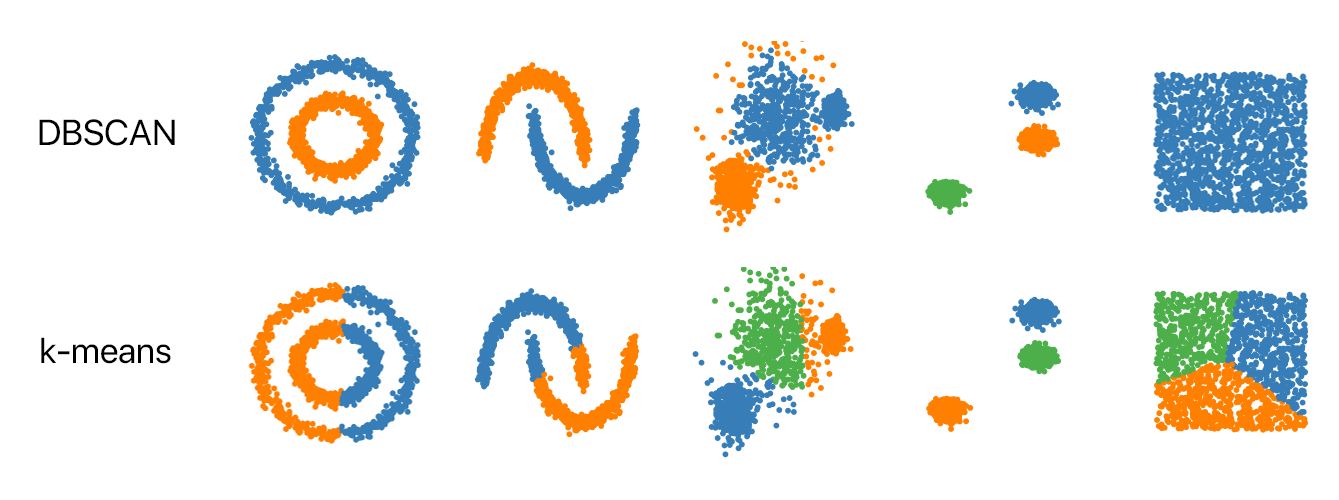
\includegraphics[width=0.5\textwidth]{images/dbscanVSkmeans.png}
    \captionsetup{width=0.6\textwidth}
    \caption{A comparison showing DBSCAN's ability to identify non-spherical clusters, in contrast to K-Means.}
    %\caption{DBSCAN Clustering Compared to K-Means: DBSCAN can identify clusters of arbitrary shapes and effectively handle noise, while K-Means tends to form spherical clusters and is sensitive to outliers.}
    \label{fig:dbscan_vs_kmeans}
\end{figure}

Key Parameters in DBSCAN:
\begin{itemize}
    \item eps ($\epsilon$): The maximum distance between two samples for one to be considered as in the neighborhood of the other.
    \item MinPts: This is the minimum number of points required within the eps radius to form a dense region. 
\end{itemize}
%1. eps: defines the radius of the neighborhood around a data point. Commonly determined with a k-distance graph Analysis. 
%Choosing the ips is Critical: If eps is too small most points will be classified as noise and if it is too large clusters may merge and the algorithm may fail to distinguish between them.
%2. MinPts: This is the minimum number of points required within the eps radius to form a dense region. 
%For most cases a minimum value of MinPts = 3 is recommended


These characteristics make DBSCAN exceptionally well-suited for analyzing real-world crime pattern.
This approach is validated by recent research: Chen et al. \cite{chen2019exploring} successfully utilized an extension of DBSCAN to detect crime hotspots from historical theft records %, validating its effectiveness in this domain

\subsection{Real-time Risk Assessment Systems}%or relevance to risk prediction
% Current approaches, GPS-based risk scoring, challenges in real-time implementation
Real-time geospatial risk assessment is the practical application of crime hotspot forecasting in operational safety systems.
While traditional approaches rely on static crime databases and predetermined risk zones, the challenge lies in integrating GPS-enabled systems to continuously process  spatial data  to calculate immidiate risk score.
\\This is the evolution from static hotspot analysis systems to active safety systems.






\section{Vocal Signal Processing for Distress Detection}
\label{vocal_processing_theory}
In real world emergencies, vocal cues such as tone, pitch, and specific keywords can provide critical 
insights into a person's state of distress. This section explores the theoretical foundations of vocal signal processing: 
Speech Emotion Recognition (SER) for emotional states detection %for detecting emotional states from audio signals, 
,Automatic Speech Recognition (ASR) for speech transcription% for transcribing spoken words 
and Natural Language Processing (NLP) for intent analysis. %for analyzing the transcribed text for intent and risk assessment.


\subsection{Speech Emotion Recognition (SER)}%emotion recognition from speech
\label{ser}
Speech contains important information beyond the words themselves, such as the speacker's emotion, pitch and tone.
Speech Emotion Recognition (SER) is the field of study focused on automatically identifying the emotional state of a speaker from their voice by analyzing acoustic and prosodic features—such as pitch, tone, and energy—to classify emotions like anger, happiness, or fear.
\\The process begins with feature extraction, a foundational concept, where meaningful data is derived from the raw audio signal, often using preprocessing  tools like \textbf{Librosa} \cite{librosa}.%todo cite it
\\Modern SER systems employ transformer-based architectures like \textbf{Wav2Vec 2.0} \cite{NEURIPS2020_92d1e1ebWav2Vec} 
which is a self-supervised model that demonstrates superior performance through pre-training on diverse audio data followed by task-specific fine-tuning.
\\For instance, research has shown that Wav2Vec 2.0 can reach an accuracy of 79.58\% on the IEMOCAP benchmark\cite{wang2022finetunedwav2vec20hubertbenchmark},% [Wang et al., 2022], %todo here we cite the paper fl okhrin we cite the offical documentation
validating its selection as a robust theoretical foundation for the distress detection module.


\subsection{Automatic Speech Recognition (ASR)}%speech-to-text conversion
\label{asr}
Automatic Speech Recognition (ASR) is the process of converting spoken language into written text, enabling machines to understand and process human speech.
The Progress in speech recognition has been energized by the development of unsupervised pre-training techniques exemplified by Wav2Vec 2.0 \cite{NEURIPS2020_92d1e1ebWav2Vec} (See \ref{ser}).  
This suggests that while unsupervised pre-training has improved the quality of audio encoders dramatically, the lack
of an equivalently high-quality pre-trained decoder, combined with a recommended protocol of dataset-specific fine
tuning, is a crucial weakness which limits their usefulness and robustness.  

For this, OpenAI implemented \textbf{Whipser}, \cite{pmlr-v139-radford21aWhisper} a Transformer-based model trained on a massive 680,000 hours of diverse audio, enabling it to perform robustly in a zero-shot setting without  
Reaserchers have also worked on a bench of versions of Whisper focusing on more epochs while adding, SpecAugment Stochastic Depth, or BPE Dropout, forming a family of Tiny, Medium, Large architectures\dots \cite{pmlr-v139-radford21aWhisper}

%Whisper models, which are trained on a broad and diverse distribution of audio and evaluated in a zero-shot setting,  
Whisper models could potentially match human behavior much better than existing systems.
To assert their efficiency, comparaisons between  Whisper models with both human performance
 and standard fine-tuned ML models were done. Whisper showed better transcription over all ML models and was close to that of professional human transcribers.
\begin{figure}[h!] % placement options: h=here, t=top, b=bottom, p=page
    \centering
    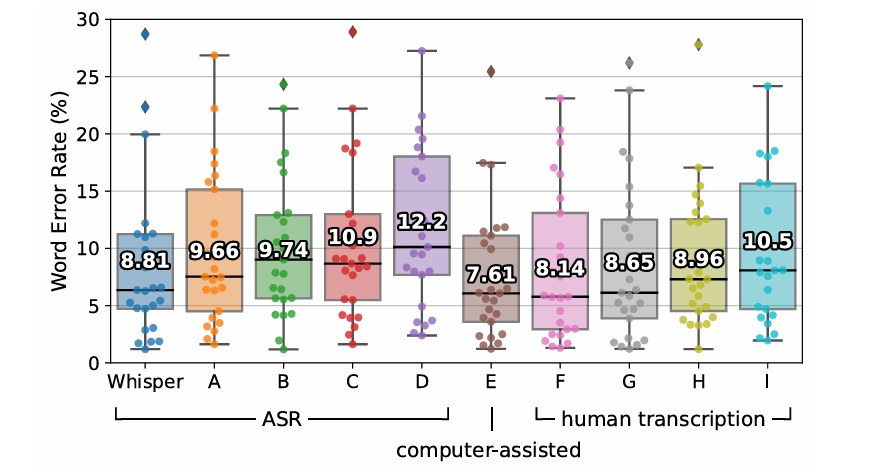
\includegraphics[width=0.5\textwidth]{images/whisper_vs_others.png}
    %\captionsetup{width=0.6\textwidth}
    \caption{Whisper's performance is close to that of professional human transcribers.}
    \label{fig:whisper_vs_others}
\end{figure}
\\In this context, it is important to note that Whisper, fine-tuned with Arabic datasets, showed impressive performance: 
It reached a WER of  81.8 on the TARIC dataset (vs95.3 for Wav2vec2.0), and 74.1 and 85.9 on respectively Tun SO and TunCS datasets.\cite{abdallah2023leveragingdatacollectionunsupervised}

\subsection{Natural Language Processing (NLP) for Intent Analysis}% intent analysis from transcribed speech
\label{sec:nlp_intent}
Natural Language Processing (NLP) is the final stage of the vocal analysis pipeline, tasked with analyzing the transcribed text from the ASR module to determine user intent in order to assess risk for distress detection.
The theory behind NLP for intent analysis relies on Transformer-based language models, notably \textbf{BERT} (Bidirectional Encoder Representations from Transformers), proven with highly effectiveness for text classification\cite{devlin-etal-2019-bert}.
\\BERT's architecture enables fine-tuning for specific tasks like intent recognition, where it identifies keywords or phrases indicative of distress.
\\A state of the art example is \textbf{TunBERT}, a model created by fine-tuning BERT on a culturally specific dataset : The T-HSAB dataset: the first Tunisian Hate Speech and Abusive dataset \cite{10.1007/978-3-030-32959-4_18THSAB}, enabling it to classify dialect-specific expressions, enhancing intent analysis for Tunisian Speech.

\section{Machine Learning for Behavioral Anomaly Detection}
\label{sec:behavioral_theory}
Behavioral anomaly detection levarages ML to create a personnalized model to identify deviations in a user's routine, indicating dangerous situations. This approach enables real-time safety in Tunisian context. The following section explores unsupervised profiling, anomaly scoring and supervised classification techniques.

\subsection{Unsupervised Profiling of User Routines}
\label{sec:unsupervised_profiling}
The foundation of the behavioral analysis module is the unsupervised profiling of a user's routines from raw spatiotemporal data. 
This process aims to build a personalized baseline of "normal" behavior without requiring any pre-labeled examples of incidents. 
The state-of-the-art approach for this task involves two key theoretical concepts:

Spatial Dimension:density-based clustering identifies geographically significant locations. The \textbf{OPTICS} (Ordering Points To Identify the Clustering Structure) \cite{304187OPTICS}
 algorithm is a powerful, state-of-the-art method for this task :
 \\ Unlike older methods like K-Means, OPTICS does not require the number of clusters to be  known beforehand. 
 It excels at discovering clusters of arbitrary shape, can handle noise, and adapt to varying point densities--
making it ideal for GPS traces in order to identify a user's routine "hotspots" such as home, work,\dots.


Temporal dimension: routines are modeled using frequency distributions. 
By analyzing the timestamps of a user's location history, the system builds probability models at different time scales:time of day,  the day of the week. 
This allows learning a user's unique temporal "pattern of life \cite{1339268pattern}," establishing a baseline for detecting unusual activity when a user deviates from their learned routine.%todo citation ib bib file 


\subsection{ Anomaly Scoring as a Measure of Deviation}
\label{sec:anomaly_scoring}
Anomaly scoring quantifies the degree of deviation from established behavioral baselines. The theoretical foundation involves measuring statistical distance between observed behaviors and learned normal patterns across multiple dimensions.

Spatial anomaly detection employs \textbf{distance-based} metrics, including \textbf{Euclidean} and \textbf{geodesic} distance measures, to assess positional deviations from routine locations %todo\cite{chandola2009anomaly}.

Temporal anomalies are typically identified through \textbf{statistical} approaches using \textbf{probability distributions}, where events occurring during periods of historically low frequency receive higher anomaly scores.

State-of-the-art techniques incorporate dynamic thresholding to adapt to evolving user patterns, addressing the challenge of concept drift in behavioral modeling  by enhancing detection accuracy in dynamic environments%todo \cite{goldstein2016comparative}[Goldstein and Uchida, 2016].


\subsection{Supervised Classification for Incident Prediction}
\label{sec:supervised_classification}
Supervised classification predicts incidents from labeled data, leveraging ensemble methods like Random Forest or XGBoost to handle imbalanced datasets [Breiman, 2001; Chen and Guestrin, 2016]. 
These techniques adapt to real-time challenges, such as sparse incident data, using adaptive thresholding to improve accuracy in evolving user behavior contexts, critical for safety monitoring.

\chapter{Design and implementation}
\label{ch:4eme}
%todo we need an intro here 
%\section{System Architecture and Data management}
\section{System Architecture, Integration, and Decision Engine Overview}
\label{sec:system_architecture}
This section outlines the overall architecture of the multi-modal safety system, detailing the technical stack, data management strategies, and the design of the final decision engine.
\subsection{Overall System Architecture}
This system integrates three AI modules: geospatial analysis, vocal signal processing, and behavioral profiling, into a cohesive framework. 
Each module processes its respective data stream and combined, they form a unified risk assessment platform, as shown in figure \ref{fig:architecture}.
\begin{figure}[h!] % placement options: h=here, t=top, b=bottom, p=page
    \centering
    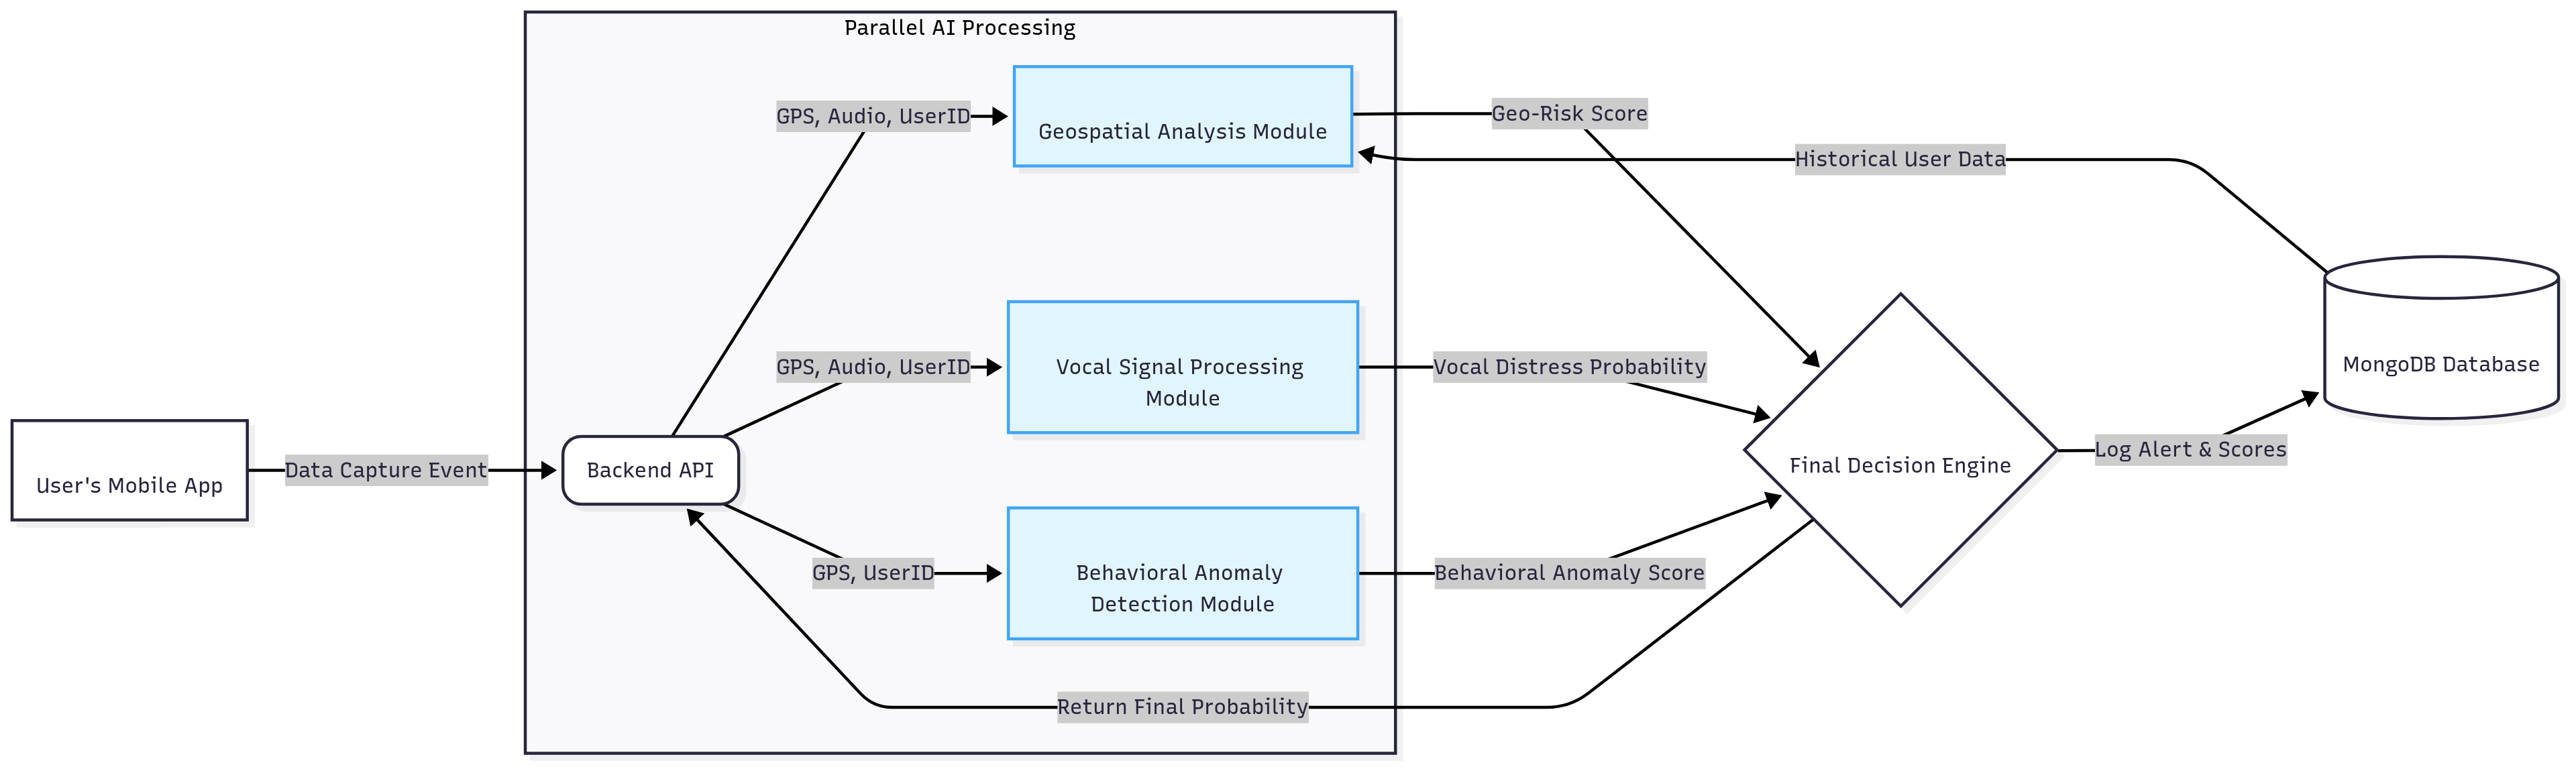
\includegraphics[width=0.9\textwidth]{images/diag5.png}
    \caption{Architecture Diagram of the System}
    \label{fig:architecture}
\end{figure}


\subsection{Final Decision Engine Design}
The decision engine integrates outputs from AI modules and non-AI inputs to declare incidents. It uses a \textbf{rule-based} approach: 
An incident is triggered if any condition is met :
%`user_anomaly_triggered` (incident_probability ≥ threshold and location_anomaly > 0.6), `geo_risk_triggered` (geo_risk_score > 0.7), `vocal_alert_triggered`, or `sos_pressed`.
\textit{SOS button pressed manually, Detected behavioral anomaly exceeding threshold, User is in a high-risk geospatial zone, Emotional distress detected in voice.}

\subsection{System Integration and API Design}
To integrate the AI-based backend with the user-facing mobile application, 
a well-defined API was designed in order to decouple the internal AI logic from the client-side application.

The system exposes a RESTful API. It supports two primary modes of operation: a single, on demand analysis for
  discrete or high-priority events, and a continuous periodic mode for ongoing safety assurance.

%the /process: which listens for incoming data "capture" events from user devices, orchestrates the entire analysis pipeline, and returns a final, consolidated risk assessment.

\subsubsection{On-demand API Endpoint}
This API is designed to handle high-priority events, such as when a user presses an SOS button on their device.%wearable
The user presses the button in a genuine emergency, triggering an immediate analysis of their current context.
The API endpoint expects a POST request with a JSON body formatted as follows:
\textbf{Endpoint:} \verb|POST /sos/<user_id>/<device_id>/<lat>/<long> |
\begin{lstlisting}[style=jsonstyle-compact]
{
  "user_id": "string",
  "device_id": "string",
  "latitude": "float",
  "longitude": "float",
  "audio_file_path": "string",
  "sos_pressed": "boolean"
}
\end{lstlisting}

\subsubsection{API Response Body}
Upon successful analysis, the API returns a JSON object with the final risk assessment:

\begin{lstlisting}[style=jsonstyle-compact]
{
  "incident_probability": 0.92,
  "is_incident": true,
  "geospatial_risk": 0.85,
  "vocal_distress_probability": 0.95,
  "behavioral_anomaly_score": {
    "location": 0.98,
    "hour": 0.75,
    "weekday": 0.20
  }
}
\end{lstlisting}

\subsubsection{Automated Periodic Risk Assessment}
For continuous safety monitoring, the system relies on a server-side scheduling mechanism to regularly trigger a check for each user at regular intervals (every 15 minutes).
This is implemented using a cron job that sends a POST request to the same /process endpoint.

\subsection{Technical stack and tools used}
\label{technical}
The system leverages a robust technical stack to enable real-time distress detection:
%This section provides an overview of the key frameworks, libraries, and tools used, grouped by their functional role within the project's architecture.

%\subsubsection{Backend Development and API}
\textbf{Backend :}
\begin{itemize}
    \item Python 3.9: The core programming language for backend logic, including data processing, model inference, and API handling, selected for its extensive ecosystem of data science and machine learning libraries.
    \item Flask: A micro web framework used to build and serve RESTful API endpoints, chosen for its lightweight, modular design ideal for mobile integration.
\end{itemize}

\textbf{Database :}
\begin{itemize}
\item MongoDB: A NoSQL document-oriented database for storing semi-structured data like user profiles and location histories, with native geospatial query support for real-time analysis.
\item PyMongo: The official Python driver used to interact with the MongoDB database.
\end{itemize}

\textbf{Machine Learning and Data Science :}
% The core AI capabilities of the system were built using a suite of industry-standard data science libraries from data preprocessing to the training and deployment of the final classification models.

\begin{itemize}

\item Scikit-learn: The foundational machine learning library, used for implementing both the DBSCAN for density-based clustering and the RandomForestClassifier for incident prediction.
\item PyTorch: A deep learning framework used to fine-tune advanced models in the vocal analysis pipeline, such as Wav2Vec 2.0.
\item NumPy \& Pandas: The workhorse libraries for all numerical computation and data manipulation, used in data preprocessing and feature engineering.
\item Librosa: A specialized library for audio analysis, used for preprocessing audio files for the vocal processing module.
\end{itemize}

\textbf{Specialized AI Models :}
% In addition to foundational libraries, the project integrated state-of-the-art, pre-trained models to handle the most complex tasks, leveraging the extensive work of the broader AI research community.
\begin{itemize}
\item OpenAI's Whisper: The model used for robust Automatic Speech Recognition.
%\item Hugging Face Transformers: The library used to access and implement pre-trained models like \textbf{Wav2Vec 2.0 }for Speech Emotion Recognition and \textbf{TunBERT} for NLP-based intent analysis.
\item Wav2Vec 2.0: A self-supervised Hugging Face Transformer used for SER, levaraged to detect emotional states from vocal patterns.
\item TunBERT: A BERT-based Hugging Face Transformer fine-tuned on Tunisian Arabic datasets for NLP-based intent analysis.%model
\end{itemize}

\subsection{Data Management and Preprocessing}
\label{sec:data_management}
Data management and preprocessing support the systems data pipeline for real-time analysis.
The data storage is handled by MongoDB, chosen for its ideal characteristics mentioned in \ref{technical}, with two main collections:
\begin{itemize}
    \item \texttt{users\_collection}: Stores user information, such as profiles and registered devices.
    \item \texttt{locations\_collection}: Acts as the main event log, storing capture events with their: timestamp, location, and payload from the decision engine.
\end{itemize}
%MongoDB serves as the primary database, storing user profiles and event logs through dedicated collections managed via custom database functions.

The preprocessing includes: \\
\textbf{Cleaning:} supports missing coordinates, invalid vocal inputs, and noisy ASR text.\\
\textbf{Preprocessing:} includes Librosa feature extraction (pitch, energy,..) for vocal data, geospatial normalization for geo-risk scoring, and tokenization for TunBERT's intent analysis, 
\\  Key challenges include sparse Tunisian geospatial data and complex Arabic NLP.
%Key challenges includesparse Tunisian geospatial data and complexities in Arabic NLP processing, requiring specialized handling approaches.

%\subsubsection{Data Storage}
%The system uses \textbf{MongoDB} for all data persistence.
%This choice was driven by its flexible schema, which is ideal for storing varied user data, and critically, its native support for high-performance \textbf{geospatial queries}, a core requirement for the location-based analysis modules. The primary database collections include:
%This choice was driven by its ideal characteristics, as discussed in \ref{technical}.
%The database collections include:

%\subsection{Final Decision Engine Design }

\section{Implementation of the Geospatial Analysis Module}
\label{geospatial_implementation}
\subsection{Data acquisition and Preprocessing}
Due to outdated National Police Crime Statistics(2015), the geospatial risk model was trained on a dataset of crime incidents in Tunisia, called ACLED \cite{raleigh2010acled} specific to Tunisia.

Preprocessing involved cleansing to extract latitude and longitude pairs, removing outliers with null values, and normalizing data using \texttt{StandardScaler} from \texttt{scikit-learn} library.
\subsection{Spatial Clustering Implementation}
The model was trained using DBSCAN \ref{sec:dbscan_theory} from \texttt{scikit-learn} to cluster high-risk zones. 
The parameters: epsilon (0.5) and min\_samples (5) were tuned dynamically on a validation set in order to get the best distribution of clusters.
Figure \ref{fig:Clusters_heatmap} illustrates the cluster distribution over Tunisia. See \ref{sec:geospatial_res} for result analysis .


%\subsection{Geospatial Risk Score and Integration}%or Integration and Performance Evaluation
\subsection{Risk Score Calculation and Integration}
%How cluster outputs are translated into risk scores.
%How these scores feed into the decision engine.
%Any performance or edge-case considerations.
%\subsection{Integration and Performance Evaluation}
The geospatial module role is to translate the user's live GPS coordinates into an immediate, actionable risk score  through a trained cluster model:

Incoming live latitude and longitude coordinates are first transformed using the same \textit{StandardScaler} that was fitted on the original training data. This ensures that the live point is evaluated in the same feature space as the model's clusters.

The system calculates the distance from the user's normalized coordinate to the centroid of every pre-computed risk cluster, identifying the single nearest high-risk cluster.

The \textit{geo\_risk\_score} is then calculated using a distance-decay function:
\\If the user is within a cluster's core radius \textit{(eps)}: They are assigned a high base score, which is weighted by the historical severity and frequency of incidents in that specific cluster. Otherwise, The  score decreases exponentially based on their distance from the edge.

The model achieved 82\% precision on a test set with latency compatible with our project's real-time alert requirements.

\section{Implementation of the Vocal Signal Processing Pipeline}
\subsection{Vocal Data Preprocessing}
All incoming audio data requires a critical preprocessing step to ensure compatibility with the pre-trained analysis models. Using the \textbf{Librosa} library, each audio file is loaded and resampled to a consistent \textbf{16kHz} format, matching the required input specifications of the Whisper and Wav2Vec 2.0 models.
 thsab: This dataset contains thousands of manually annotated Tunisian comments from social media, capturing the specific vocabulary 
and expressions used in high-stress or abusive contexts

\subsection{Integration of SER, ASR, and NLP for Distress Detection}%or multi-modal vocal analysis nhbbklmt pipeline : max 3 jomlett.
\label{integration_ser_asr_nlp}
%todo this is only a draft was in the sota chapter
The integration of Speech Emotion Recognition (SER), Automatic Speech Recognition (ASR), and Natural Language Processing (NLP) forms a comprehensive vocal analysis pipeline for distress detection.
This multi-modal approach leverages the strengths of each component to provide a robust assessment of vocal distress signals.
\\The SER module analyzes the emotional tone of the speech, identifying signs of fear or anxiety that may indicate distress.
Sim ultaneously, the ASR module transcribes the spoken words into text, capturing the explicit content of the communication.
Finally, the NLP module processes the transcribed text to extract intent and context, identifying keywords or phrases that suggest an emergency situation.
By combining emotional cues with linguistic analysis, this integrated pipeline enhances the accuracy and reliability of distress detection, ensuring that both the emotional state and the verbal content are considered in the assessment.



\section{Implementation of the Behavioral Profiling Module} % or the Behavioral Anomaly Detection Module or the Machine Learning Module
\subsection{Behavioral Data Preprocessing}
The behavioral module's data is prepared in two distinct stages:
\begin{itemize}
    \item \textbf{For User Profiling}: To build a user's behavioral profile, their historical location data is fetched from the \texttt{locations\_collection} and filtered to include events from the last 30 days.
    \item \textbf{For Incident Classification}: To train the final \texttt{RandomForestClassifier}, a labeled dataset is created from past alerts. For each alert, a feature vector is constructed from the four anomaly scores (location, hour, weekday, month), and the target label is set based on the \texttt{is\_incident} field.
\end{itemize}
%todo le faite quon a synthetisé de la data pour new users ? si je me rappelle bien, en t cas comment we handled new users
\subsection{Implementation of Unsupervised Profiling}
\label{sec:unsupervised_implementation}
%todo this is a draft
% Purpose: Detail the practical execution of unsupervised profiling.
%
% What to write:
% 1. Describe data source (`locations_collection`) and processing.
% 2. Explain applying DBSCAN/OPTICS to identify hotspots (e.g., home, work).
% 3. Mention frequency distribution use in `db_functions.py`.
Unsupervised profiling in Hydatis uses locations\_collection` GPS data, processed via 
DBSCAN to identify routine hotspots like home or work. OPTICS handles arbitrary shapes, 
while frequency distributions in `db\_functions.py` model temporal 
patterns (e.g., weekday mornings), building a "pattern of life" for anomaly detection.


\subsection{Anomaly Scoring }
Anomaly scoring, the 2nd stage of the behavioral analysis, quantifies the degree of deviation of a new, live event from the user's established profile. This is accomplished by calculating an anomaly score—a numerical
 value representing how "unusual" an event is. This score is not a single value, but rather a vector of scores, with each element corresponding to a different dimension of the user's behavior.
For spatial deviations, the score is derived from the geometric distance between a user's current coordinates and the centroids of their known routine locations. A greater distance corresponds to a 
higher anomaly score, indicating the user is in a location they frequent less often.
For temporal deviations, the score is based on the principle of inverse frequency. 
An event's timestamp (e.g., the hour of the day) is compared against the learned frequency distributions from the user's profile. Activities occurring at times with low historical probability 
(e.g., being active at 3 AM for a user who is typically home) are assigned a significantly higher anomaly score. By combining these scores, the system creates a rich, multi-dimensional feature vector that 
captures the full context of a user's deviation from their normal "pattern of life."

%\section{Final Decision Engine and System Integration}
%this may be merged with the first section (dont know shkoun shyemshi bahtha sahbou ( hawka naamlou referencing lel sections elli will tailor the details if nkaddmou el decision engine kbal les ai modules))

\chapter{Results and Discussion}
\label{ch:results_and_disc}

\section{Evaluation and Results}
\label{sec:res}
\subsection{Geospatial}
\label{sec:geospatial_res}
Figure \ref{fig:Clusters_heatmap} illustrates the cluster distribution to put in the appendixacross Tunisia, highlighting urban risk areas. See Discussion for result analysis.
\begin{figure}[h!] % placement options: h=here, t=top, b=bottom, p=page
    \centering
    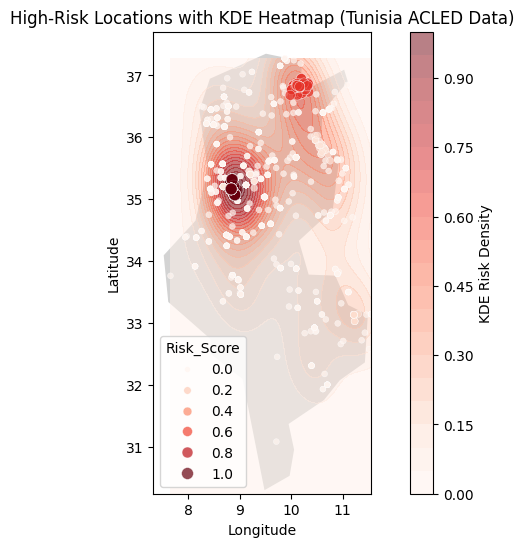
\includegraphics[width=0.5\textwidth]{images/high_risk_locations_heatmap_tunisia_acled_data.png}
    \caption{High Risk Locations Heatmap of Tunisia based on the ACLED Data}
    \label{fig:Clusters_heatmap}
\end{figure}





\section{Discussion}

Edge cases, including sparse rural data coverage, were mitigated using synthetic data generation, though further validation is needed (see Discussion).






%\section*{Conclusion}
%\section{Conclusion}
\chapter*{Conclusion and perspectives}
\addcontentsline{toc}{chapter}{Conclusion and perspectives}
\markboth{Conclusion and perspectives}{}

\begin{appendix}
\chapter{Appendix 1}
Insert your appendixes here if you need.
\end{appendix}

%\spacing{1}
\bibliographystyle{unsrt}
\bibliography{references}
\end{document}